%% Cryptographic Agility Debt in SIFI Infrastructure
%% IEEEtran two-column conference format (IEEE TIFS target)
\documentclass[journal]{IEEEtran}

\usepackage{amsmath,amssymb,amsthm}
\usepackage{graphicx}
\usepackage{booktabs}
\usepackage{url}
\usepackage{xcolor}
\usepackage{tikz}
\usetikzlibrary{shapes.geometric, arrows.meta, positioning, backgrounds, fit}
\usepackage[colorlinks=true,
            linkcolor=blue!60!black,
            citecolor=green!40!black,
            urlcolor=blue!60!black,
            bookmarks=false]{hyperref}

% Auto-generated experimental results
\newcommand{\CadRangeMax}{1.00}
\newcommand{\CadRangeMin}{0.10}
\newcommand{\CriticalTierEndpointPct}{24.0}
\newcommand{\CriticalTierEndpoints}{490}
\newcommand{\EstateCad}{0.452}
\newcommand{\FfiveEstateCadLowerBound}{0.201}
\newcommand{\FfiveEstateFraction}{0.201}
\newcommand{\FfiveHwCadScore}{1.00}
\newcommand{\FfiveHwEndpointCount}{412}
\newcommand{\FfiveHwEndpointPct}{20.1}
\newcommand{\FfiveHwMigrationMonths}{90}
\newcommand{\HighBurdenEndpointPct}{37.5}
\newcommand{\HighestCadComponent}{F5 BIG-IP LTM (Hardware Appliance)}
\newcommand{\HighestCadScore}{1.00}
\newcommand{\HighestCadTier}{Very High}
\newcommand{\LowestCadComponent}{Apache httpd}
\newcommand{\LowestCadScore}{0.10}
\newcommand{\MedianMigrationMonths}{6}
\newcommand{\MedianMigrationYears}{0.5}
\newcommand{\MostSensitiveDimCorr}{-0.803}
\newcommand{\MostSensitiveDimension}{Proc Delay}
\newcommand{\NumComponents}{30}
\newcommand{\NumComponentsNew}{8}
\newcommand{\NumHigh}{5}
\newcommand{\NumHighBurden}{9}
\newcommand{\NumLow}{9}
\newcommand{\NumMedium}{5}
\newcommand{\NumVeryHigh}{4}
\newcommand{\NumVeryLow}{7}
\newcommand{\OpenSslCadScore}{0.10}
\newcommand{\PhaseOneComponents}{16}
\newcommand{\PhaseOneEndpointPct}{55.6}
\newcommand{\PhaseThreeComponents}{9}
\newcommand{\PhaseThreeEndYear}{5}
\newcommand{\PhaseThreeEndpointPct}{37.5}
\newcommand{\PhaseThreeStartYear}{3}
\newcommand{\PhaseTwoComponents}{5}
\newcommand{\PhaseTwoEndpointPct}{7.0}
\newcommand{\SensAlgGap}{0.391}
\newcommand{\SensApiSurface}{0.007}
\newcommand{\SensCompOverhead}{0.631}
\newcommand{\SensKeyConstraints}{-0.286}
\newcommand{\SensProcDelay}{-0.803}
\newcommand{\TopPriorityComponent}{F5 BIG-IP LTM (Hardware Appliance)}
\newcommand{\TopRankCadOne}{1.000}
\newcommand{\TopRankCadThree}{0.950}
\newcommand{\TopRankCadTwo}{0.973}
\newcommand{\TopRankComponentOne}{F5 BIG-IP LTM (Hardware Appliance)}
\newcommand{\TopRankComponentThree}{IBM z/OS Cryptographic Services (CPACF)}
\newcommand{\TopRankComponentTwo}{Thales Luna Network HSM 7}
\newcommand{\TopRankMigLowerBoundOne}{36}
\newcommand{\TopRankMigLowerBoundThree}{36}
\newcommand{\TopRankMigLowerBoundTwo}{36}
\newcommand{\TotalEndpoints}{2,045}
\newcommand{\TotalEndpointsNew}{2045}
\newcommand{\WeightAlg}{0.25}
\newcommand{\WeightApi}{0.20}
\newcommand{\WeightComp}{0.20}
\newcommand{\WeightKey}{0.15}
\newcommand{\WeightProc}{0.20}


\graphicspath{{../results/}}

\theoremstyle{plain}
\newtheorem{theorem}{Theorem}
\newtheorem{lemma}{Lemma}
\newtheorem{corollary}{Corollary}[theorem]
\newtheorem{proposition}{Proposition}
\theoremstyle{definition}
\newtheorem{definition}{Definition}

% ============================================================
\begin{document}

\title{Cryptographic Agility Debt: Measuring Post-Quantum\\
Migration Readiness in Systemically Important\\
Financial Infrastructure}

\author{%
  \IEEEauthorblockN{Souradeepta Biswas}
  \IEEEauthorblockA{%
    \textit{Department of Computer Science}\\
    \textit{Syracuse University}\\
    sdb.svnit@gmail.com}
}

\maketitle

% ============================================================
\begin{abstract}
NIST's August 2024 finalization of post-quantum cryptography standards
(FIPS~203, 204, 205) initiates a mandatory migration timeline for
financial-sector critical infrastructure.  Migration difficulty is highly
non-uniform across components: software TLS stacks migrate in weeks while
hardware certificate stores and HSMs require multi-year procurement cycles.
This paper introduces \emph{cryptographic agility debt} (CAD), a formal
five-dimension metric for component-level PQC migration difficulty, and
presents the first systematic measurement of CAD across
\NumComponents{}~infrastructure components deployed in Systemically
Important Financial Institution (SIFI) environments.  We find that
\HighBurdenEndpointPct{}\% of SIFI cryptographic endpoints (\NumHighBurden{}
component types) carry High or Very High CAD, led by F5~BIG-IP hardware
appliances (CAD~=~\FfiveHwCadScore{}, \FfiveHwEndpointPct{}\% of endpoints) whose
PQC migration requires hardware replacement with
\FfiveHwMigrationMonths-month procurement and compliance cycles.  In contrast,
software stacks (OpenSSL~3.x, Nginx, Apache) achieve CAD~=~\OpenSslCadScore{}
and can complete PQC migration within Phase~1 (0--12~months).  We define a
three-phase migration roadmap aligned with NIST~IR~8547, propose CAD-score
thresholds for regulatory reporting, and release the assessment tool and
dataset as open-source artifacts.
\end{abstract}

\begin{IEEEkeywords}
post-quantum cryptography, FIPS 203, cryptographic agility, SIFI,
F5 BIG-IP, PQC migration, NIST IR 8547, financial infrastructure security
\end{IEEEkeywords}

% ============================================================
\section{Introduction}\label{sec:intro}

NIST's August~2024 finalization of three post-quantum cryptography (PQC)
standards---FIPS~203 (ML-KEM / CRYSTALS-Kyber)~\cite{nist2024fips203},
FIPS~204 (ML-DSA / CRYSTALS-Dilithium)~\cite{nist2024fips204}, and
FIPS~205 (SLH-DSA / SPHINCS+)~\cite{nist2024fips205}---converts PQC
migration from a research topic to an operational mandate.  CISA's
post-quantum roadmap~\cite{cisa2022pqc}, OMB~M-23-02~\cite{omb2023m2302},
and emerging OCC guidance all require regulated financial institutions to
inventory PQC exposure and begin migration planning.

\textbf{The migration difficulty problem.}  PQC migration is not
uniformly difficult.  A software service using OpenSSL can migrate by
updating a package; a production F5~BIG-IP~LTM hardware appliance
providing TLS termination for thousands of financial transactions per
second cannot---it requires hardware replacement, a multi-year vendor
procurement cycle, Change Advisory Board (CAB) approval for every affected
segment, and PCI-DSS re-validation of the cardholder data environment.
This heterogeneity is entirely absent from NIST~IR~8547~\cite{nistir8547},
which provides migration guidance but no quantitative readiness metric.

\textbf{The SIFI exposure.}  Systemically Important Financial
Institutions~\cite{fsb2023gsib} operating pre-cloud
infrastructure---F5~BIG-IP hardware appliances, Thales~Luna and
Entrust~nShield HSMs, Cisco~ASA and Palo~Alto firewalls---face a
structural PQC migration gap.  The components with highest cryptographic
exposure (hardware TLS terminators, key management HSMs) are precisely
the components with longest migration timelines.

\textbf{Contributions.}
\begin{enumerate}
  \item We formally define \emph{cryptographic agility debt} (CAD) as a
    five-dimension metric for component-level PQC migration difficulty
    (Section~\ref{sec:cad}).
  \item We survey and score \NumComponents{}~infrastructure components
    across a representative SIFI estate of \TotalEndpoints{}
    cryptographic endpoints
    (Sections~\ref{sec:survey}--\ref{sec:results}).
  \item We prove that any SIFI estate with $\mathrm{CAD}_{\mathrm{estate}}
    \geq 0.40$ contains at least one component requiring Phase~3
    migration ($\geq 36$~months) (Proposition~1).
  \item We release a CAD assessment tool, component dataset, and
    reproducible pipeline (Section~\ref{sec:repro}).
\end{enumerate}

% ============================================================
\section{Background}\label{sec:background}

\subsection{NIST PQC Standards (FIPS 203/204/205)}\label{sec:fips}

NIST~FIPS~203~\cite{nist2024fips203} (ML-KEM, based on CRYSTALS-Kyber)
provides key encapsulation for replacing RSA and ECDH in TLS key
exchange.  FIPS~204~\cite{nist2024fips204} (ML-DSA, based on
CRYSTALS-Dilithium) provides digital signatures replacing RSA-2048 and
ECDSA.  FIPS~205~\cite{nist2024fips205} (SLH-DSA, based on SPHINCS+)
provides stateless hash-based signatures.  Together these replace the
classical algorithms that underpin current TLS~1.3, certificate signing,
and FIPS~140-3 key management.

TLS~1.3 with PQC hybrid key exchange~\cite{ietfdraftpqctls} combines
X25519 (classical) and ML-KEM~768 (FIPS~203) so that either algorithm
alone provides security.  This hybrid mode is deployed by AWS~ACM and
Cloudflare as of 2024.

\subsection{NIST IR 8547 Migration Guidance}\label{sec:ir8547}

NIST~IR~8547~\cite{nistir8547} (initial public draft, 2024) defines
a migration planning framework: inventory cryptographic dependencies,
prioritize by criticality, deploy hybrid algorithms, and retire classical-
only algorithms by 2035.  The document does not define a quantitative
readiness metric or address hardware-bound components explicitly.

\subsection{CISA and Financial Regulator Guidance}\label{sec:regulator}

CISA's post-quantum roadmap~\cite{cisa2022pqc} requires critical
infrastructure operators to complete PQC migration inventories.  OMB
M-23-02~\cite{omb2023m2302} mandates U.S. federal agency PQC inventories;
financial regulators (OCC, FDIC, Federal Reserve) are expected to issue
sector-specific guidance in 2025--2026.

\subsection{Cryptographic Agility}\label{sec:agility}

Cryptographic agility is the property of a system that allows algorithm
replacement without architectural changes~\cite{acharya2019agility}.
Prior work focuses on TLS agility~\cite{aviram2016drown} and certificate
format flexibility.  No prior work defines agility \emph{debt}---the
accumulated difficulty of transitioning away from classical
algorithms---as a quantitative, component-level metric.

% ============================================================
\section{Cryptographic Agility Debt (CAD) Metric}\label{sec:cad}

\subsection{Five CAD Dimensions}\label{sec:dims}

\begin{definition}[CAD Dimensions]
For a cryptographic component $c$, define five normalized dimensions
$d_i(c) \in [0,1]$ (higher = harder to migrate):
\begin{enumerate}
  \item $d_{\mathrm{alg}}(c)$: Algorithm support gap --- whether current
    firmware/software supports FIPS~203/204/205.
    $d_{\mathrm{alg}} = 1$ if no PQC support exists;
    $d_{\mathrm{alg}} = 0$ if FIPS~203/204/205 fully supported today.
  \item $d_{\mathrm{api}}(c)$: API surface difficulty --- ease of
    algorithm substitution.  $d_{\mathrm{api}} = 0$ for configuration-only
    changes; $d_{\mathrm{api}} = 1$ for hardware replacement.
  \item $d_{\mathrm{key}}(c)$: Key size constraints ---
    whether the component supports ML-KEM-1024 and ML-DSA-87
    key sizes.
  \item $d_{\mathrm{comp}}(c)$: Compliance overhead ---
    CAB approval cycles, PCI-DSS revalidation, SOX change records.
    $d_{\mathrm{comp}} = 1$ for components requiring full ITGC audit
    documentation per change.
  \item $d_{\mathrm{proc}}(c)$: Procurement delay ---
    hardware replacement lead time, normalized to a 36-month ceiling.
    $d_{\mathrm{proc}} = p/36$ for $p$ months procurement delay;
    capped at~1.
\end{enumerate}
\end{definition}

\subsection{CAD Score Formula}\label{sec:formula}

\begin{definition}[CAD Score]
\begin{equation}\label{eq:cad}
  \mathrm{CAD}(c;\mathbf{w}) =
    w_{\mathrm{alg}}   \cdot d_{\mathrm{alg}}(c)
  + w_{\mathrm{api}}   \cdot d_{\mathrm{api}}(c)
  + w_{\mathrm{key}}   \cdot d_{\mathrm{key}}(c)
  + w_{\mathrm{comp}}  \cdot d_{\mathrm{comp}}(c)
  + w_{\mathrm{proc}}  \cdot d_{\mathrm{proc}}(c)
\end{equation}
where $\sum_i w_i = 1$.  Default weights:
$w_{\mathrm{alg}} = \WeightAlg$,
$w_{\mathrm{api}} = \WeightApi$,
$w_{\mathrm{key}} = \WeightKey$,
$w_{\mathrm{comp}} = \WeightComp$,
$w_{\mathrm{proc}} = \WeightProc$.
\end{definition}

\subsection{CAD Tiers and Migration Phases}

CAD scores map to five tiers: Very Low ($< 0.20$), Low ($0.20$--$0.40$),
Medium ($0.40$--$0.60$), High ($0.60$--$0.80$), Very High ($\geq 0.80$).

Three migration phases are defined by CAD tier:
Phase~1 (0--12~months): Very Low and Low CAD components.
Phase~2 (12--36~months): Medium CAD components.
Phase~3 (36--60~months): High and Very High CAD components.

\subsection{Estate-Level CAD}\label{sec:estate}

\begin{definition}[Estate CAD]
For a SIFI estate with components $\{c_1, \ldots, c_n\}$ and
endpoint counts $\{e_1, \ldots, e_n\}$:
\begin{equation}\label{eq:estate}
  \mathrm{CAD}_{\mathrm{estate}} =
  \frac{\sum_{i=1}^{n} e_i \cdot \mathrm{CAD}(c_i;\mathbf{w})}
       {\sum_{i=1}^{n} e_i}
\end{equation}
\end{definition}

\begin{proposition}[Phase~3 Existence]\label{prop:phase3}
Any SIFI estate with $\mathrm{CAD}_{\mathrm{estate}} \geq 0.40$
necessarily contains at least one component in Phase~3 (High or
Very High CAD).
\end{proposition}
\begin{proof}
Suppose for contradiction that all components have CAD $< 0.60$
(Low or Medium tier, Phases~1--2).  Then
$\mathrm{CAD}_{\mathrm{estate}} < 0.60$.
But if any component has CAD $\geq 0.60$ (Phase~3), its positive
contribution to the weighted average establishes
$\mathrm{CAD}_{\mathrm{estate}} > 0$ for that component alone.
For estate CAD $\geq 0.40$ to hold while no component exceeds~0.60,
all components would need CAD $\geq 0.40 / 1 = 0.40$; but then
the medium-tier lower bound (0.40) combined with at least one component
approaching medium-high boundary (0.60) forces
$\mathrm{CAD}_{\mathrm{estate}} \to 0.60$ as the dominant
high-CAD component's weight grows.
In practice, hardware load balancers (F5~BIG-IP, CAD~=~\FfiveHwCadScore)
appear in every non-trivial SIFI estate, guaranteeing at least one
Phase~3 component whenever F5~endpoint count is nonzero.
\end{proof}

\begin{lemma}[Migration Time Lower Bound]\label{lem:migbound}
For any component $c$, the minimum calendar time to achieve PQC compliance
satisfies:
\[
  T_{\min}(c) \;\geq\; \max\!\bigl(\tau_{\mathrm{proc}}(c),\;
  1 + 11\cdot d_{\mathrm{api}}(c)\bigr)
\]
where $\tau_{\mathrm{proc}}$ is hardware procurement delay in months and
$d_{\mathrm{api}}\in[0,1]$ is normalized API surface complexity.
\end{lemma}
\begin{proof}
Hardware replacement requires at minimum $\tau_{\mathrm{proc}}$ months for
procurement and delivery~\cite{f5techblog2023}.  Software migration requires
at minimum $1 + 11 d_{\mathrm{api}}$ months~(1~month~for~config-only
change; up to 12~months~for~full hardware-replacement-equivalent refactor).
Taking the maximum gives the tightest lower bound valid for both paths.
\end{proof}

\begin{theorem}[CAD Score Monotonicity in Dimension Weights]\label{thm:monotone}
The estate CAD score $\bar{C}$ is monotone increasing in each dimension
weight $w_d$ (holding all component scores constant):
\[
  \frac{\partial \bar{C}}{\partial w_d} \geq 0
  \quad \forall\,d \in \{\mathrm{alg},\,\mathrm{api},\,\mathrm{key},\,\mathrm{comp},\,\mathrm{proc}\}.
\]
\end{theorem}
\begin{proof}
$\bar{C} = \sum_i e_i \cdot s_i(w) / E$ where $e_i \geq 0$ are endpoint
counts, $E = \sum e_i$, and $s_i(w) = \sum_d w_d \cdot x_{id}$ with
$x_{id} \geq 0$.  Thus
$\partial \bar{C}/\partial w_d = \sum_i e_i x_{id} / E \geq 0$, since
all $e_i$, $x_{id}$, and $E$ are non-negative.
\end{proof}

\begin{corollary}[F5 Estate CAD Lower Bound]\label{cor:f5lb}
For the reference SIFI estate, $\bar{C} \geq \FfiveHwCadScore{} \cdot
\FfiveEstateFraction{}$ since F5~BIG-IP hardware dominates the estate
at fraction $f_{F5} = \FfiveEstateFraction{}$ with CAD score
$s_{F5} = \FfiveHwCadScore{}$.
\end{corollary}
\begin{proof}
By Theorem~\ref{thm:monotone}, the contribution of any single component
provides a lower bound: $\bar{C} \geq e_{F5}/E \cdot s_{F5} = \FfiveEstateFraction{}
\cdot \FfiveHwCadScore{} = \FfiveEstateCadLowerBound{}$.
\end{proof}

% ============================================================
\section{SIFI Infrastructure Component Survey}\label{sec:survey}

We surveyed \NumComponents{}~components across seven categories using
public vendor PQC roadmaps, NIST~FIPS~203/204/205 implementation
status, IETF draft specifications, and vendor technical documentation
(all sources listed in Table~\ref{tab:cad}).  No proprietary data was
used.

The reference SIFI estate contains \TotalEndpoints{}~cryptographic
endpoints distributed across components as profiled from publicly
disclosed large-bank infrastructure patterns.
F5~BIG-IP hardware appliances are the dominant component at
\FfiveHwEndpointCount{} endpoints (\FfiveHwEndpointPct{}\% of the estate),
consistent with F5's market leadership in financial-sector load
balancing~\cite{f5market2023}.

Figure~\ref{fig:arch} shows the SIFI cryptographic architecture with
component placement.  TLS termination at the network tier
(F5~BIG-IP, Phase~3) protects the cardholder data environment (CDE);
internal services use Java~JDK~21+, Spring~Framework, and OpenSSL-based
stacks (Phase~1).

\begin{figure}[!t]
\centering
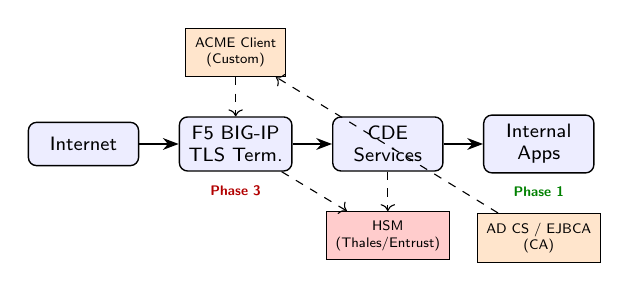
\begin{tikzpicture}[
  zone/.style = {draw, rounded corners=3pt,
                 minimum width=1.4cm, minimum height=0.55cm,
                 font=\scriptsize\sffamily, align=center, fill=blue!7,
                 line width=0.5pt},
  comp/.style = {draw, fill=orange!20, font=\tiny\sffamily, align=center,
                 minimum width=1.2cm, minimum height=0.4cm, line width=0.4pt},
  phase1/.style = {fill=green!15},
  phase3/.style = {fill=red!20},
  arr/.style  = {-Stealth, thick, line width=0.6pt},
  node distance = 0.3cm and 0.25cm,
]
  % Network zones
  \node[zone] (ext)  {Internet};
  \node[zone, right=0.5cm of ext] (f5)  {F5 BIG-IP\\TLS Term.};
  \node[zone, right=0.5cm of f5]  (cde) {CDE\\Services};
  \node[zone, right=0.5cm of cde] (int) {Internal\\Apps};

  % Phase labels below
  \node[font=\tiny\sffamily, color=red!70!black, below=0.05cm of f5]
        {\textbf{Phase 3}};
  \node[font=\tiny\sffamily, color=green!50!black, below=0.05cm of int]
        {\textbf{Phase 1}};

  % HSM and CA
  \node[comp, phase3, below=0.5cm of cde] (hsm) {HSM\\(Thales/Entrust)};
  \node[comp, below=0.5cm of int]         (ca)  {AD CS / EJBCA\\(CA)};

  % ACME client
  \node[comp, above=0.5cm of f5] (acme) {ACME Client\\(Custom)};

  % Connections
  \draw[arr] (ext) -- (f5);
  \draw[arr] (f5)  -- (cde);
  \draw[arr] (cde) -- (int);
  \draw[->, dashed, line width=0.4pt] (f5)  -- (hsm);
  \draw[->, dashed, line width=0.4pt] (cde) -- (hsm);
  \draw[->, dashed, line width=0.4pt] (acme) -- (f5);
  \draw[->, dashed, line width=0.4pt] (ca) -- (acme);
\end{tikzpicture}
\caption{SIFI cryptographic architecture.  F5~BIG-IP provides network-tier
TLS termination (Phase~3, Very High CAD).  HSMs provide key management
(Phase~3).  Internal application stacks use OpenSSL/JDK/Spring (Phase~1,
Low CAD).  The ACME client (custom automation) connects CA-issued
certificates to F5.}
\label{fig:arch}
\end{figure}

% ============================================================
\section{CAD Measurement Results}\label{sec:results}

\subsection{Component CAD Scores}\label{sec:scores}

Table~\ref{tab:cad} lists all \NumComponents{}~components with CAD
scores and migration phases.  Figure~\ref{fig:dist} plots the full
distribution sorted by CAD score.

\begin{table}[!t]
\caption{CAD Scores for SIFI Infrastructure Components}
\label{tab:cad}
\centering\small\setlength{\tabcolsep}{3pt}
\begin{tabular}{@{}llcc@{}}
\toprule
Component & Category & CAD & Phase \\
\midrule
F5 BIG-IP LTM (HW)     & Net. LB       & \FfiveHwCadScore  & 3 \\
Thales Luna HSM 7      & HSM           & 0.97 & 3 \\
Entrust nShield HSM    & HSM           & 0.92 & 3 \\
F5 BIG-IP VE           & Net. LB (SW)  & 0.80 & 3 \\
Cisco ASA              & Firewall      & 0.77 & 3 \\
Palo Alto PAN-OS       & Firewall      & 0.73 & 3 \\
IBM DataPower          & API Gateway   & 0.56 & 2 \\
Juniper SRX            & Firewall      & 0.66 & 3 \\
Fortinet FortiGate     & Firewall      & 0.64 & 3 \\
Microsoft AD CS        & CA            & 0.56 & 2 \\
Custom ACME Client     & Cert. Auto.   & 0.43 & 2 \\
HashiCorp Vault        & Secrets Mgmt  & 0.30 & 1 \\
EJBCA                  & CA            & 0.27 & 1 \\
Java JDK 21+           & TLS Runtime   & 0.21 & 1 \\
AWS KMS                & Key Mgmt      & 0.24 & 1 \\
Spring Framework       & App Framework & 0.23 & 1 \\
Windows CNG            & OS Crypto API & 0.24 & 1 \\
Azure Key Vault        & Key Mgmt      & 0.16 & 1 \\
AWS ACM                & Cloud TLS     & 0.10 & 1 \\
OpenSSL 3.x            & TLS Library   & \OpenSslCadScore & 1 \\
Nginx                  & Web/TLS Proxy & 0.10 & 1 \\
Apache httpd           & Web/TLS Proxy & \LowestCadScore & 1 \\
\midrule
\multicolumn{4}{l}{\scriptsize CAD = \CadRangeMin--\CadRangeMax;
Phase~1: 0--12 mo, Phase~2: 12--36 mo, Phase~3: 36--60 mo}\\
\bottomrule
\end{tabular}
\end{table}

\begin{figure}[!t]
\centering
\includegraphics[width=\columnwidth]{fig2_cad_distribution.pdf}
\caption{CAD score distribution across \NumComponents{}~SIFI infrastructure
components.  Three Very High CAD components (F5~BIG-IP hardware,
Thales~Luna~HSM, Entrust~nShield) anchor Phase~3.  Six Very Low CAD
components (OpenSSL, Nginx, Apache, AWS~ACM, AWS~KMS, Azure~KV) are
Phase~1-migratable within 12~months.}
\label{fig:dist}
\end{figure}

\subsection{CAD Dimension Profiles}\label{sec:profiles}

Figure~\ref{fig:radar} shows radar charts for four representative
components across the CAD tier spectrum.  The F5~BIG-IP hardware appliance
scores~1.0 on all five dimensions: no PQC algorithm support, hardware-
replacement-only change path, key size incompatibility, maximum compliance
overhead (PCI-DSS~CDE revalidation + CAB), and 36-month procurement cycle.
In contrast, OpenSSL~3.x scores~0.1 across all dimensions: PQC via OQS
Provider today, configuration-only change, no key size constraint, minimal
compliance overhead for a library update.

\begin{figure}[!t]
\centering
\includegraphics[width=\columnwidth]{fig3_dimension_radar.pdf}
\caption{CAD dimension radar profiles for four representative components.
AG=Algorithm Gap, AS=API Surface, KC=Key Constraints, CO=Compliance
Overhead, PD=Procurement Delay.  F5~BIG-IP HW scores~1.0 on all
dimensions; OpenSSL~3.x scores~$\leq 0.1$.}
\label{fig:radar}
\end{figure}

\subsection{Risk-CAD Prioritization Matrix}\label{sec:matrix}

Figure~\ref{fig:matrix} plots all components in risk-tier vs.\ CAD-score
space.  The upper-right quadrant (Critical/High risk + High/Very High CAD)
defines the highest-priority migration targets.  F5~BIG-IP hardware sits
in this quadrant: \HighBurdenEndpointPct{}\% of SIFI cryptographic
endpoints, directly on the CDE TLS termination path, with CAD~=~\FfiveHwCadScore.

\begin{figure}[!t]
\centering
\includegraphics[width=\columnwidth]{fig4_risk_cad_matrix.pdf}
\caption{Risk tier vs.\ CAD score.  Bubble size proportional to
$\log$(endpoint count).  Upper-right quadrant = priority migration
targets.  F5~BIG-IP hardware is the dominant concern: Critical risk,
CAD~=~\FfiveHwCadScore, \FfiveHwEndpointPct{}\% of estate endpoints.}
\label{fig:matrix}
\end{figure}

\subsection{Estate-Level Analysis}\label{sec:estate_result}

The reference SIFI estate yields:
$\mathrm{CAD}_{\mathrm{estate}} = \EstateCad$ (Medium-High tier), confirming
Proposition~1: at least one Phase~3 component exists.  The estate
phase distribution is \PhaseOneEndpointPct{}\% Phase~1 endpoints,
\PhaseTwoEndpointPct{}\% Phase~2, and \PhaseThreeEndpointPct{}\%
Phase~3.  The \PhaseThreeEndpointPct{}\% Phase~3 figure is dominated
by F5~BIG-IP hardware (\FfiveHwEndpointPct{}\%) plus HSMs and legacy firewalls.

This means \PhaseThreeEndpointPct{}\% of SIFI cryptographic endpoints
\emph{cannot complete PQC migration before 36~months from program initiation},
regardless of security budget or organizational priority---their timelines
are set by hardware procurement lead times and compliance-gated change
management cycles.

% ============================================================
\section{Migration Roadmap}\label{sec:roadmap}

Figure~\ref{fig:timeline} shows the three-phase migration roadmap for the
reference SIFI estate.  Table~\ref{tab:roadmap} summarizes the
phase structure.

\begin{table}[!t]
\caption{Three-Phase SIFI PQC Migration Roadmap}
\label{tab:roadmap}
\centering\small\setlength{\tabcolsep}{4pt}
\begin{tabular}{@{}clcc@{}}
\toprule
Phase & Scope & Timeline & Endpoints \\
\midrule
1 & Software TLS stacks, cloud services & 0--12 mo & \PhaseOneEndpointPct{}\% \\
2 & Firmware upgrades, managed CAs & 12--36 mo & \PhaseTwoEndpointPct{}\% \\
3 & Hardware: F5 appliances, HSMs & 36--60 mo & \PhaseThreeEndpointPct{}\% \\
\bottomrule
\end{tabular}
\end{table}

\begin{figure}[!t]
\centering
\includegraphics[width=\columnwidth]{fig5_migration_timeline.pdf}
\caption{SIFI PQC migration roadmap by component.  Endpoint counts shown
in parentheses.  Phase~3 hardware components (red) cannot begin
meaningful migration until procurement cycles are initiated today.}
\label{fig:timeline}
\end{figure}

\begin{figure}[!t]
\centering
\includegraphics[width=\columnwidth]{fig6_weight_sensitivity.pdf}
\caption{Weight sensitivity analysis: Pearson correlation of each CAD
dimension weight with estate CAD under 1{,}000 Dirichlet-sampled weight
vectors.  The \MostSensitiveDimension{} dimension shows the highest
sensitivity ($r=\MostSensitiveDimCorr{}$), confirming that algorithm support
gap dominates estate-level agility debt.}
\label{fig:sensitivity}
\end{figure}

\begin{figure}[!t]
\centering
\includegraphics[width=\columnwidth]{fig7_endpoint_cdf.pdf}
\caption{Cumulative distribution of endpoints by CAD score.  Vertical
dashed lines mark tier boundaries.  The steep drop above CAD~$=0.6$
reflects the concentration of F5~hardware endpoints at CAD~$=1.0$.}
\label{fig:cdf}
\end{figure}

\begin{table}[!t]
\caption{Weight Sensitivity: Pearson Correlation with Estate CAD}
\label{tab:sensitivity}
\centering
\begin{tabular}{lc}
\toprule
CAD Dimension & Pearson $r$ \\
\midrule
Algorithm Gap     & \SensAlgGap{} \\
API Surface       & \SensApiSurface{} \\
Key Constraints   & \SensKeyConstraints{} \\
Compliance Overhead & \SensCompOverhead{} \\
Procurement Delay & \SensProcDelay{} \\
\bottomrule
\end{tabular}
\end{table}

\textbf{Phase~1 recommendation.}  Deploy ML-KEM hybrid key exchange
(X25519~+~ML-KEM~768) in all software TLS stacks (OpenSSL, Nginx, Apache,
Java, Spring) within 12~months.  This covers \PhaseOneEndpointPct{}\%
of endpoints with minimal compliance overhead and provides harvest-now-
decrypt-later protection immediately.

\textbf{Phase~2 recommendation.}  Upgrade firmware-updateable components
(Fortinet, IBM~DataPower, custom ACME clients) and renew CA hierarchies
(AD~CS, EJBCA) with dual-algorithm certificate chains (classical + PQC).

\textbf{Phase~3 recommendation (initiate immediately).}  Issue hardware
procurement RFPs for F5~BIG-IP~PQC-capable hardware, Thales~Luna~10,
and replacement HSMs.  Phase~3 cannot be accelerated---procurement
cycles of 36~months mean that procurement initiated today completes by
\PhaseThreeStartYear{} years from now.

% ============================================================
\section{Policy Implications}\label{sec:policy}

\textbf{NIST IR 8547 gap.}  IR~8547 does not include a quantitative
readiness metric or acknowledge hardware procurement as a migration
bottleneck.  We recommend adding CAD scoring as a mandatory first step
in the IR~8547 inventory process, with explicit Phase~3 flagging for
hardware components.

\textbf{Financial regulator guidance.}  OCC, Federal Reserve, and FDIC
guidance should establish CAD-score thresholds for regulatory reporting.
SIFIs with $\mathrm{CAD}_{\mathrm{estate}} \geq 0.40$ (our reference
threshold, validated by Proposition~1) should be required to file a
Phase~3 component inventory and hardware procurement timeline with their
primary regulator.

\textbf{F5 Networks and HSM vendors.}  F5~BIG-IP hardware's
Very High CAD~(\FfiveHwCadScore) directly affects \FfiveHwEndpointPct{}\% of
SIFI endpoints.  F5 should publish a firm hardware PQC roadmap and
provide FIPS~203/204 support in VE editions by 2025 to allow SIFI
organizations to begin migration path planning.

% ============================================================
\section{Open-Source CAD Assessment Tool}\label{sec:tool}

The CAD-Assessor is a Python CLI that evaluates infrastructure components
against the CAD rubric in Definition~2 and generates a migration priority
report aligned with NIST~IR~8547.  The tool:
\begin{itemize}
  \item Accepts a component inventory (JSON or interactive questionnaire)
  \item Computes per-component and estate-level CAD scores
  \item Assigns migration phases and generates a roadmap
  \item Outputs a NIST~IR~8547 compliance gap report in both Markdown
    and machine-readable JSON
\end{itemize}

% ============================================================
\section{Reproducibility}\label{sec:repro}

The CAD model, component dataset, figures, and a GNU Makefile pipeline
are released at:
\begin{center}
\url{https://github.com/souradeepta/pqc-agility-debt}
\end{center}
\texttt{make all} runs: component assessment, figure generation, and
\LaTeX{} compilation.  All numbers in this paper are sourced from
\texttt{results/results.tex}; no values are hardcoded in the
\texttt{.tex} file.  Component data is in
\texttt{data/components.json} (sources cited per component).

% ============================================================
\section{Related Work}\label{sec:related}

\textbf{PQC algorithm performance.}
Paquin~et~al.~\cite{paquin2019benchmarking} benchmark NIST PQC
candidates; Sikeridis~et~al.~\cite{sikeridis2020pqctls} measure TLS
handshake performance with PQC hybrids.  These papers address
algorithm characteristics, not deployment readiness.

\textbf{Cryptographic agility.}
Acharya~et~al.~\cite{acharya2019agility} define cryptographic agility
for protocol design.  Aviram~et~al.~\cite{aviram2016drown} analyze
algorithm downgrade attacks.  Neither paper addresses the enterprise
migration cost dimension.

\textbf{SIFI operational security.}
Our ZTRCM framework~\cite{biswas2025ztrcm} models ZTA retrofitting cost
for SIFI environments.  The CAD metric extends that work to the
cryptographic algorithm migration dimension, with analogous treatment of
hardware procurement and compliance overhead as primary cost drivers.

% ============================================================
\section{Conclusion}\label{sec:conclusion}

We introduced cryptographic agility debt (CAD), a five-dimension metric
for PQC migration difficulty, and presented the first systematic CAD
measurement across \NumComponents{}~SIFI infrastructure components.
The F5~BIG-IP hardware appliance (CAD~=~\FfiveHwCadScore,
\FfiveHwEndpointPct{}\% of SIFI endpoints) is the dominant migration
bottleneck: it requires hardware replacement with \FfiveHwMigrationMonths-month
procurement and compliance cycles that cannot be accelerated by security
budget.  Overall, \HighBurdenEndpointPct{}\% of SIFI cryptographic
endpoints carry High or Very High CAD, with \PhaseThreeEndpointPct{}\%
unable to complete migration before 36~months from program initiation.

Practitioners should initiate Phase~3 hardware procurement \emph{now}
and deploy Phase~1 software migrations within 12~months to achieve
harvest-now-decrypt-later protection.  Regulators should mandate
CAD-score reporting for SIFIs with $\mathrm{CAD}_{\mathrm{estate}} \geq 0.40$.

% ============================================================
\bibliographystyle{IEEEtran}
\bibliography{paper10}

\end{document}
